\documentclass[sigplan,10pt,twocolumn,letterpaper]{article}
%\settopmatter{printfolios=true}
\special{papersize=8.5in,11in}
\setlength{\pdfpagewidth}{8.5in}
\setlength{\pdfpageheight}{11in}
\usepackage[noheadfoot,
            left=1in,right=1in,top=1in,bottom=1in,
            columnsep=0.25in
            ]{geometry}
\usepackage[small,compact]{titlesec}
\usepackage[font={small,bf}]{caption}
\usepackage[nolineno,noindent,norules]{lgrind}
\usepackage{tightenum}
\usepackage{float}
\usepackage{xspace}
\usepackage{times,pifont}
\usepackage{mathptmx}
\usepackage{subfig,graphics,graphicx,color}
\usepackage{multirow}
\usepackage{dblfloatfix} %% correctly orders single- and double-col figures
\usepackage{hyphenat}
\usepackage{mathrsfs}
\usepackage{subfig}
\usepackage{amssymb,amsmath,centernot}
\usepackage{lastpage}
\usepackage{flushend}
\usepackage{hhline}
\usepackage{authblk}
\usepackage[hyphens]{url}
\usepackage{adjustbox}
\usepackage{algorithm}
\usepackage[noend]{algpseudocode}
%\newcommand{\doi}{XXXXXX}


%%% ================= START of SOSP '13 template ================= 
% \makeatletter
% 
% \def\ftype@copyrightbox{8}
% \def\@copyrightspace{
% \@float{copyrightbox}[b]
% \begin{center}
% \setlength{\unitlength}{1pc}
% \begin{picture}(20,6.0) 
% \put(0,3){\parbox{\columnwidth}{\scriptsize
% 
% %*** SAMPLE. AUTHOR PUT SUPPLIED TEXT HERE ****
% 
% \noindent
% \rule{6.0 cm}{0.2pt}\\
% Permissiondddd to make digital or hard copies of part or all of this work 
% for personal or classroom use is granted without fee provided that
% copies are not made or distributed for profit or commercial advantage 
% and that copies bear this notice and the full citation on the first
% page. Copyrights for third-party components of this work must be
% honored.  For all other uses, contact the Owner/Author. 
% 
% \vspace{\baselineskip}\noindent
% Copyright is held by the Owner/Author(s).\\
% \textit{SOSP'15}.\\
% ACM XXXXXXX.
% 
% \noindent
% http://dx.doi.org/\doi}
% }
% \end{picture}
% \end{center}
% \end@float}
% 
% \def\maketitle{\par
%  \begingroup
%    \def\thefootnote{\fnsymbol{footnote}}
%    \def\@makefnmark{\hbox
%        to 0pt{$^{\@thefnmark}$\hss}}
%      \twocolumn[\@maketitle]
% \@thanks
%  \endgroup
%  \setcounter{footnote}{0}
%  \let\maketitle\relax
%  \let\@maketitle\relax
%  \gdef\@thanks{}\gdef\@author{}\gdef\@title{}\gdef\@subtitle{}\let\thanks\relax
%  \@copyrightspace}
% 
% \makeatother

%%% ================= END of SOSP '13 template ================= 



%\newcommand{\comment}[1]{}
\frenchspacing
%\doublespacing
%%%%%%%%%%%%%%%%%%%%%%%%%%%%
%     macro

% paper-specific definitions
\newcommand{\sys}[0]{Argus\xspace}

\newcommand{\xxx}{\mbox{\textsc{XXXXX}}\xspace}
\newcommand{\wechat}{\mbox{\textsc{XXXXXX}}\xspace}
%\newcommand{\mytitle}[0]{\textbf {\sys: Understanding Livelocks Through Full-System Tracing}}
\newcommand{\mytitle}[0]{\textbf {\sys: Understanding App Behavior Through Full-System Tracing}}

\newcommand{\mykeywords}[0]{Performance debug}

%%%%%%%%%%%%%%%%%%%%%%%%%%%%%%%%%%%%%%%%%%%%%%%%%%%%%%%%%%%%%%%%%
% hyperref stuff

\usepackage[square,comma,numbers,sort]{natbib}
\usepackage{hypernat}
\usepackage[draft]{hyperref}
%\usepackage{hyperref}

%% fill in pdf info here
\hypersetup{%
colorlinks=false,
pdfborder={0 0 0},
pdftitle={\mytitle},
pdfkeywords={\mykeywords},
bookmarksnumbered,
pdfstartview={FitH},
urlcolor=cyan,
pdfpagelabels=true,
pdfdisplaydoctitle=true,
}%

%\usepackage{breakurl}
%\usepackage[all]{hypcap}
%\renewcommand{\url}{\burl}

%%%%%%%%%%%%%%%%%%%%%%%%%%%%%%%%%%%%%%%%%%%%%%%%%%%%%%%%%%%%
% Some NICE fonts

\newfont{\BIG}{cminch}                             %--- One-inch font
\newfont{\sfbHuge}{cmssbx10 scaled\magstep5}       %-- 25pt sans serif bold
\newfont{\sfbLarger}{cmssbx10 scaled\magstep3}   %-- 12+pt sans serif boldd
\newfont{\sfblarger}{cmssbx10 scaled\magstep2}   %-- 12+pt sans serif bold
\newfont{\sfblarge}{cmssbx10 scaled\magstep1}      %-- 12pt sans serif bold
\newfont{\sfbeleven}{cmssbx10 scaled\magstephalf}  %-- 11pt sans serif bold
\newfont{\sfb}{cmssbx10}                           %-- 10pt sans serif bold
\newfont{\sfeight}{cmss8}                          %-- 8pt sans serif

%%%%%%%%%%%%%%%%%%%%%%%%
%   space tweaking

%\textwidth = 6.5 in
%\textheight = 9.0 in
%\setlength{\topmargin}{-.5in}

%\headheight = 0.0 in
%\headsep = 0.0 in
%\parskip = 0.2in
%\parindent = 0.0in

\renewcommand{\topfraction}{0.95}
\addtolength{\textfloatsep}{-0.1in}
%\addtolength{\floatsep}{0.025in}
\renewcommand\floatpagefraction{.9}
%\renewcommand\bottomfraction{.9}
\renewcommand\textfraction{.1}
%\renewcommand\footnotetextcopyrightpermission[1]{}
\renewcommand{\algorithmicrequire}{\textbf{Input:}}

\setlength{\parindent}{9pt}

% Rescue
\makeatletter
\def\v#1{{\mbox{\fontfamily{cmtt}\fontsize{\f@size}{\f@size}\selectfont #1}}}

\newcommand{\messaging}[0]{\textsc{Messaging}\xspace}
\newcommand{\pthread}[0]{\mbox{Pthreads}\xspace}

% In short.
\newcommand{\eg}{{e.g. }}
\newcommand{\ie}{{i.e. }}
\newcommand{\etc}{{etc}}
\newcommand{\para}[1]{\vspace{.00in}\noindent{\bf #1}}
\newcommand{\wrt}{{w.r.t. }}
\newcommand{\cf}{{cf. }}
\newcommand{\etal}{{et al. }}

% operations.
\newcommand{\psynchcvwait}[0]{\v{psynch\_cv\_wait()}\xspace}
\newcommand{\send}[0]{\v{send()}\xspace}
\newcommand{\recv}[0]{\v{recv()}\xspace}

% stats.
\newcommand{\proxy}{\mbox{\textsc{Proxy}}\xspace}
\newcommand{\serviceA}{\mbox{\textsc{Service A}}\xspace}

\def\LGfsize{\footnotesize}
%\pagestyle{empty}

\begin{document}

% Hack for: Package caption Error: No float type 'copyrightbox' defined.
%\newcounter{copyrightbox}

\date{}

%\title{\mytitle\\
%\rm \Large Title For Paper}
\title{\mytitle}

\author[+]{\hspace{0 mm}\fontsize{10}{10}\selectfont SOSP
2019 submission \#XX}
\maketitle

\begin{sloppypar}
\begin{abstract}
%Althought many efforts are made to eliminate performance bugs,
%optimizations in both software and hardware,
%they still exist every computing platforms. 
%Spinning beachball is an indicator used to imply performance bugs in Mac.
%However, debugging in such cases are still hard.
%The user should know where the app gets stuck and what exactly causes the hanging(root cause).
%Using lldb to reproduce such bug is impossible due to the high latency caused by the tool.
%It hard to tell if the showing beach ball indicates a performance bug or not.
%Moreover, multiple processing and multiple threading are common used in current system.
%The root cause of the hanging is not straitforward.
%The long latency in the UI thread may caused by a worker thread in the App, event due to the wait on daemons. 
%We proposed XXX which leverage the trace tool by Apple to monitor system wide events 24X7.
%After collecting the data we analyze and tell the user where the stuck redides.
%With the confined range, XXX also provide tools to further execute a conditional debugging.

\end{abstract}
\end{sloppypar}

%%%%%%%%%%%%%%%%%%%%%%%%%%%%%%%%%%%
% Add page number.
\setcounter{page}{1}
\pagenumbering{arabic}

\thispagestyle{plain}
\pagestyle{plain}
\setlength{\footskip}{20pt}
%%%%%%%%%%%%%%%%%%%%%%%%%%%%%%%%%%%

\begin{sloppypar}

%\section{Introduction} \label{sec:intro}

Today's web and desktop applications are predominantly parallel or
distributed, making performance issues in them extremely difficult to
diagnose because the handling of an external request is often spread across
many threads, processes, and asynchronous contexts instead of in one
sequential execution segment~\cite{harter2012file}. To manually reconstruct
a graph of execution segments for debugging, developers have to sift
through a massive amount of log entries and potentially code of related
application components~\cite{chen2002pinpoint, zhao2016non, xu2009detecting,
nagaraj2012structured, yuan2012conservative}. More often than not, developers
give up and resort to guessing the root cause, producing ``fixes'' that
sometimes make the matter worse. For instance, a bug in the Chrome browser
engine causes a spinning cursor in macOS when a user switches the input
method~\cite{chromiumbugreport}, was first reported in 2012. Developers
attempted to add timeouts to work around the issue. Unfortunately, the bug has
remained open for seven years and the timeouts obscured diagnosis further.

Prior work proposed what we call \emph{Causal tracing}, a powerful technique
to construct request graphs automatically~\cite{reynolds2006pip, fonseca2007x,
benjamin2010dapper, zhang2013panappticon, ravindranath2012appinsight}. It
does so by inferring (1) the beginning and ending boundaries of the execution
segments (vertices in the graph) involved in handling a request; and (2) the
causality between the segments (edges)---how a segment causes others to do
additional handling of the request. Compared to debuggers such as \spindump that
capture only the current system state, causal tracing is effective at aiding
developers to understand complex causal behaviors and pinpoint the root causes
for real-world performance issues.

Prior causal tracing systems all assume certain programming idioms to automate
inference. For instance, if a segment sends a message, signals a condition
variable, or posts a task to a work queue, it wakes up additional execution
segment. Prior systems assume that wake-ups reflect causality. Similarly, they
assume that the execution segment, from the beginning of a callback invocation
to the end, is entirely for handling related work in a request. Unfortunately,
based on our study and experience of building a causal tracing system for macOS,
we find that modern applications violate these assumptions. Hence, the request
graphs computed by causal tracing are inaccurate in several ways.

First, an inferred segment can be larger than the actual event handling segment
due to batch processing. Specifically, for performance, an application or its
underlying frameworks may bundle together work on behalf of multiple requests
with no clear distinguishing boundaries. For instance, WindowServer in macOS
sends a reply for a previous request and receives a message for the current
request using one system call \vv{mach\_msg\_overwrite\_trap}, presumably to
reduce user-kernel crossings. Second, the graphs can miss numerous causal
edges. For instance, consider data dependencies in which the code sets a flag
(\eg, ``\vv{need\_display} = 1'' in macOS animation rendering) and later
queries the flag to process a request further. This pattern is broader than
ad hoc synchronization~\cite{xiong2010ad} because data dependency occurs
even within a single thread (such as the buffer holding the reply in the
preceding WindowServer example). Although the number of these flags may be
small, they often express critical causality, and not tracing them would lead
to many missing edges in the request graph. However, without knowing where
the flags reside in memory, a tool would have to trace all memory operations,
incurring prohibitive overhead and adding many superfluous edges to the request
graph. Third, inferred edges can be superfluous because wake-ups do not
necessarily reflect causality. Consider an \vv{unlock()} operation waking up an
thread waiting in \vv{lock()}. This wake-up can just be happenstance and the
developer's intent is mutual exclusion. However, the two operations can also
enforce a causal order.

We believe that, without fully understanding of application semantics, request
graphs computed by causal tracing are \emph{inherently} inaccurate and both
over- and under-approximate reality. Although developer annotations can help
improve accuracy~\cite{reynolds2006pip, fonseca2007x}, modern applications use
more and more third-party libraries, whose source code is not available. Given
the frequent use of custom synchronizations, work queues, and data flags in
modern applications, it is hopeless to count on manual annotations to ensure
accurate capture of request graphs.

In this work, we present \xxx, a dramatically different approach in the design
space of causal tracing. It is desgined for tech-savvy users who are intersted
in compiling useful bug reports for their daily use applications, whose source
codes are often not available. As opposed to full manual schema upfront for
all involved applications and daemons~\cite{barham2004using, reynolds2006pip,
fonseca2007x}, \xxx calculates an event graph for a duration of the system
execution with both true causal edges and weak ones, and enables users to
provide necessary schematic information on demand in diagnosis. Specifically, it
keeps humans in the loop, as a debugger should rightly do. \xxx queries users a
judicially few times to (1) resolve a few inaccurate edges that represent false
dependencies and (2) identify potential dependency due to data flags.

We implement \xxx in macOS, which is closed-source on its frameworks and many
applications. This closed-srouce environment therefore provides a true test
of \xxx. We address multiple nuances of macOS that complicate causal tracing,
and build a system-wide, low-overhead, always-on tracer. \xxx enables users to
optionally increase the granularity of tracing (\eg, logging call stacks and
instruction streams) by integrating with existing debuggers such as \vv{lldb}.

We evaluate \xxx on \nbug real-world, open spinning-cursor issues in widely
used applications such as Chromium browser engine and macOS System Preferences,
Installer, and Notes. The root causes of all \nbug issues were previously
unknown to us and, to a large extent, the public. Our results show that \xxx is
effective: it helps us non-developers of the applications find all root causes
of the issues, including the Chromium issue that remained open for seven years.
\xxx mostly needs only less than 3 user queries per issue but they are crucial
in aiding diagnosis. \xxx is also lightweight: its systems-wide tracing incurs
only \cpuoverhead CPU overhead overall.

%% consider adding comparison to prior approaches
%% Our techniques effectively removed false and added missing edges in the
%% event graph.  Even with our techniques, the resultant graph remain too
%% inaccurate for traditional causal tracing, but, fortunately, an average
%% of XXX user queries suffice to locate the root causes accurately.

We make the following contributions: 
\begin{enumerate}

\item We demonstrate conceptual realization that causal tracing is inherently
inaccurate, and introduce interactive approach in the design space of causal 
tracing.

\item We build \xxx, performing system-wide tracing in macOS with little
overhead, and handle several macOS trickeries that complicate causal tracing.

\item We use \xxx to diagnose real-world spinning cursors and find root causes for
performance issues that have remained open for years.

\end{enumerate}

This paper is organized as follows. In Section~\ref{sec:background}, we
introduce the causal tracing and prior works. In Section~\ref{sec:overview},
we present an overview of using \xxx and a Chromium example. In
Section ~\ref{sec:inaccuracy}, we report inherently inaccuracy
patterns observed in macOS , and Section~\ref{sec:implementation}
describes our tracing implementation and tools for user interaction.
Section~\ref{sec:eval} demonstrates the methodology and results from case
studies, as well as performance evaluation. We summarize related work
in Section~\ref{sec:related-work}, and end with conclusion in Section
~\ref{sec:conclusion}.

%\section{Background: Casual Tracing} \label{sec:background}

\begin{figure}[tb]
	\footnotesize
    \centering
	 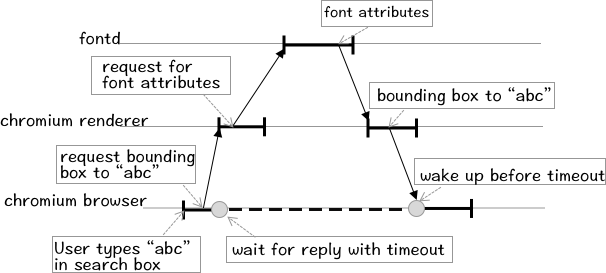
\includegraphics[width=\columnwidth]{./figures/causaltracing_example.png}
    \caption{Handling User Typing in Chromium.  The \vv{browser} and
      \vv{render} each split the work among a main thread and a worker
      thread.  Front service daemon \vv{fontd} uses thread pooling.  For
      clarity, only processes are shown, not their threads.}
    \label{fig:chromium-normal}
\end{figure}

Modern applications are often highly concurrent, spreading the handling of
an external request in multiple threads, processes, and asynchronous
contexts, each of which may multiplex on different requests.  Causal
tracing thus aims to reconnect the execution segments physically separated
in different execution contexts but logically on behalf of the same
request.  Figure~\ref{fig:chromium-normal} shows an example in Chromium,
an open-source browser engine that powers Google Chrome and, starting
recently, Microsoft Edge~\cite{chromiumurl}. When a user types a string in
Chromium, the \vv{browser} process sends an IPC message to the \vv{render}
process where the rendering view and WebKit code run, to calculate the
bounding box of the string.  \vv{render} then queries \v{fontd}, the font
service daemon, to calculate the height and length of the string in the
given font.  Once \vv{fontd} finishes, it sends an IPC reply to wake up
\vv{render} which in turn wakes up \vv{browser}.  The handling of user
typing is thus split among at least three processes and their relevant
threads, and an ideal causal tracing tool would capture these segments
(vertices) and their connections (edges) into a generalized control-flow
graph to aid developer reasoning.

Compared to tools such as \spindump that capture only the current system
state such as the call stack snapshots of each thread, causal tracing
captures the dependency path of events, enabling users to trace across
threads and processes to past events.  For instance, if \vv{render}'s
reply hangs \vv{browser}, causal tracing would enable a developer to
examine \vv{fontd}'s reply to \vv{render}, whereas the \vv{fontd} call
stack that \spindump captures at the time of the hang may be for a
completely irrelevant request.

Mechanically, to build an event graph, causal tracing tools must infer the
beginning and ending boundaries of execution segments and connect a
segment with the other segments that it creates or wakes up. Lacking
application semantics, existing tools make various assumptions to infer
segment boundaries and connections.  We select AppInsight and Panappticon,
two tools closely related to \xxx, and describe how they do so.

AppInsight is designed to help developers understand the performance
bottlenecks in mobile applications.  To infer execution segment
boundaries, it interposes on the interface between the application and
framework, and assumes that the application follows mostly the event
callback programming idiom.  The entry and exit of a callback invocation
delimit an execution segment.  If this segment installs additional
callbacks or signals a waiting thread, then AppInsight connects the
corresponding segments.

Panappticon detects performance issues in Android applications. It traces
low-level events in the Android system and libraries.  To infer execution
segment boundaries and connections, it assumes two programming idioms:
work queue and thread pooling.  For work queue, it marks the handling of a
work item as an execution segment, and connects this segment to the
segment that dispatches the work item.  For thread pooling, it marks from
the wakeup of a worker thread to the wait as an execution segment, and
connects this segment to the segment waking up the worker thread.

%% In this section, we illustrate causal tracing and prior work on it. Causal
%% tracing collects events standing for instrucions executed in CPU and generates
%% a graphical representation with traced events as vertices. Two events always
%% following a sequential constraint reflects causality, which is represented
%% as an edge. The graph helps users understand the complex causal behaviors across
%% thread/process boundaries and attribute bugs to their root causes. Prior works
%% have different definitions of vertices, edges, and root causes based on what
%% events are collected.

%% AppInsight instruments all the upcalls from the framework to the application.
%% It traces user input, display update, the begin and end of procedual call, the
%% invocation of callback function, exception and blocking events in threads. Each
%% event is reflected as a vertex in the request graph. Therefore, the request
%% graph connects (1)user input event to (2)the beginning of event handler, which
%% in turn connects to (3)the beginning of callback in background threads. The
%% vertices like (2) and (3) will connect to (4)the end of the procedual call
%% or lead to (5 )exception. Besides, they will also connect to (6)blocking for
%% signal, if the execution requires synchronization. The goal of AppInsight is to
%% help developers understand the performance bottlenecks with critical paths or
%% exception paths. It defines the root cause as the state of a function execution,
%% long blocking or exception in the application.

%% To be unobtrusive, Panappticon instruments the system to collect low-level
%% and fine grained events from libraries and kernel, including user input,
%% display update, asynchronous call and callback, inter-process comminication,
%% synchronization mechanism, and resource accounting. Every event is a vertex.
%% Panappticon connects continuous vertices which stem from atomic work in a
%% thread, \eg, a worker thread processing one task from a task queue, into an
%% execution interval. Two execution intervals are connected if the earlier
%% interval triggers the latter one. For example, a user input triggering an
%% enqueue message in the same thread reflects as an execution interval, where
%% two vertices are connected with a temperal ordering edge. In another thread,
%% dequeuing the message and submiting an asynchronous task generate another
%% execution interval. The two intervals are connected with a causal edge. With the
%% resouces analysis in every user transaction, from user input to display update,
%% Panapption speculates and manually inspect root causes from design flaws, harmful
%% interaction, to underpowered hardware.

%\section{Design}
\label{sec:design}

Our \xxx prototype is designed to debug performance issues in complex modern applications.
It performs lightweight full system tracing of every process including system calls, interprocess messages, and MacOS system daemons.
Offline, we build a graph based on thread executions, with nodes defined by per-event execution segments, and edges wherever there are temporal constraints between threads of execution.

\subsection{Use Cases}

\xxx can be used in two primary ways:
\begin{enumerate}
    \item \xxx can continuously run live in the background and collect full
    system logs. The user works as usual until a crash or performance issue is
    observed.

    \item The user can begin with a reproducible performance issue, and collect
    logs in two situations: a) a baseline situation where the program runs
    normally, and b) a spinning situation that exposes the performance issue.

\end{enumerate}
For a simple issue, like a rare segmentation fault, just having \xxx's lightweight logs may be enough to perform a diagnosis.
However, in most cases, \xxx will need to be used interactively, so the user needs to be able to reproduce the problem.
The user can request more detailed logs in several ways, reproducing the problem, and gathering enough data to narrow in even further on the problem.
The general process for interactive debugging with \xxx is as follows:
\begin{enumerate}
    \item First, the user finds the node \emph{$N_{spin}$} in the \xxx graph
    that corresponds to a hanging thread of execution. The user may leverage
    the system clock time to search for events (\eg, keystrokes).

    \item Next, the user attempts to find the node in the normal case that
    corresponds with $N_{spin}$. There will likely be many possible candidates
    at first, so the user can narrow in on specific nodes and gather more
    detailed information in that area of the program.

    \item Now, with knowledge of $N_{spin}$ and (a small number of) matching
    nodes in the normal graph, the user performs a backward slice through the
    graphs to attempt to find the defining difference between the cases. This
    difference should accurately predict whether a given log represents a
    normal or spinning case, and usually indicates quite directly the root
    cause. As before, additional information may need to be collected from
    certain points in the program to be able to distinguish between the cases.

\end{enumerate}
As shown in Figure XXX, the user's main operations are a) manual inspection of
the graph, b) performing slicing on the graph to show dependent nodes, c)
selecting a graph node to gather more information about, and d) comparing graph
slices between normal and spinning cases.

\section{Introduction}

%\section{Approach Overview}

%The \xxx prototype is designed to expose the thread relationships with temporal constraints as an graph and allow analysis toolkit built on for diagnosis.
%Workloads running on MacOS usually send requests to various sets of daemons.
%One request can take paths through multiple daemons, while one daemon can also accept a batch of comming messages and demultiplex them in a daemon thread.
%For example, the window server communicates with every application to pass the user input events and draw things on the display.
%Our framework records the system-wide activities with minimal instrumentation and constructs the thread relationship with our defined event schema built in the framework.

\subsection{Instrumentation}
The instrumentation in \xxx leverages tracing technology from Apple's event logging infrastructure.
An event consists of a timestamp, an event type name to annotate current activity, and arbitrary attributes.
One example is as the following line.

\textit{timestamp, Mach\_msg\_send, local\_port, remote\_port, ...}

The API that produces a stream of timestamped events of an event type is called a tracing point.
The goal of our Instrumentation is to attach the tracing points in significant spots where the thread state can be captured.
The code where the asynchronous task is submitted is one of the significant spots.
In the situation, the asynchronous handler should be captured from the local stack or registers in the thread.

There are three main categories of tracing points:
\begin{enumerate}
	\item Tracing points implies the relationship across thread boundaries.
	\item Tracing points identifies the requests boundaries inside a thread.
	\item Tracing points improves the comprehension of the system activity, e.g. the call stacks.
\end{enumerate}

Most of them are from the kernel which is open source and pre-existing in the current version of MacOS.
We augment them with more attributes to support our extensive use.
Libraries and frameworks providing batch processing programming paradigms are instrumented to detangle multiple requests.
We can instrument anywhere if necessary, but rarely touch the user space to allow our toolkits more general.

\subsection{Graph Construction}
In the process of graph construction, we extract the built-in event schema that indicates how a subset of events connected, and if an event acts as a delimiter, which implies a thread reaches the beginning or end of a request.
We link the threads with connections defined in the subset of events and split the threads with the implied delimiters.
A thread is split into multiple execution segments, decomplexing the execution of different requests on the thread.
Therefore, multiple graphs are generated to represent the system activities, with the execution segments mapped to the nodes and the links among them to the edges.

%%TODO: add reference of magpie and AppInsight
However, the graphs constructed with event schema is neither accurate nor complete definitely.
The missing connections may be caused by shared variables which are widely used for the synchronizations among threads but is too exhaustive to explore.
On the other hand, the delimiters are not explicit somewhere due to undocumented programming paradigms.
For example, a batch processing programming paradigm is not uncommon in current systems from user-defined server thread to the kernel thread.
Furthermore, the relationship between a thread waits, and another thread wakes it up later, are not equal to the dependency between them.
To improve the constructed graphs, we come up with an ad-hoc hardware watchpoint tool to monitor shared variables if necessary to improve the completeness, and heuristics to ensure each node is only on behalf of one request.
We present the details in the following sections.

\subsection{Analysis Toolkit}
With the graphs generated, analysis tools can be built on for various purposes, studying requests, comparison multiple executions or retrieve the bug paths.
Some design mechanism can be revealed with the graphs.
Our roughly generated graph on a toy app used particular API tells how the API gets implemented and what daemons are accessed to complete it.
For example, NSLog is implemented by sending messages to a server.
%TODO: add details here on NSLog thing
The design of the spinning cursor in MacOS is tapped by checking the path that triggers spindump.
Timestamps carried by the tracing events helps to calculate the time cost of the execution segments, as well as the blocking time of a thread on specific resources.
By checking the long execution segments or the long time blocking in UI thread, users can confine the performance anomaly to the execution interval.

\section{Built-in Event Schema}\label{section: builtin_event_schema}
Our instrumentation framework must be able to capture system events that indicate a performance anomaly, without significantly impacting performance or consuming too much storage space.
The built-in event schema simplifies the use of our system for users without expert knowledge to capture application and system state.
Trace points and other messages that do not match the schema are discarded to save disk space.
We only record events that can be used to define execution segments within threads.
During post-processing, we form temporal links between threads and split execution into segments.
% and summarize the results for the user.
We make extensive use of the tracing points added by Apple and augment them with necessary attributes in the kernel.
Libraries and Frameworks are instrumented only when necessary.

Execution segments are defined in terms of links, so we discuss links next.

\subsection{Link}
We create link from source to destination thread in the following cases:
\begin{itemize}
        \item Inter-process Communications: As mentioned in pattern P7, MacOS
        IPC uses mach\_msg with up to four threads involved in every
        communication. Every step of the communication contains a reply port
        which can be used to trace the communication, and we create a link when
        the final thread sends a message to original reply port.

        \item Thread-scheduling: Thread context switches may occur in our logs
        for multiple reasons. Except for patterns P1 and P2, we create a link
        between the yielding thread and the thread that wakes up.

        \item Timer-arm-and-fire: Timers may be registered at any point by
        passing a function pointer to a system call \texttt{mk\_timer}. When
        the timer interrupt fires, the kernel will invoke each callback
        function. We link the callback to the original thread that armed the
        timer. If the timer re-registers itself (pattern P9), we will continue
        to link future callbacks to the original registration point.

        %\item Timer-arm-and-fire: Timers are widely used in the Cocoa
        %Framework. We add tracing points in the kernel to capture the where it
        %is armed and where it is fired or canceled. The timer mechanism is
        %implemented by encapsulating the callout function in a kernel object
        %and linking/removing the object to/from the timer lists. Therefore, we
        %record the slid address of the object and the user passed in function
        %address as attributes in the kernel, which is used to connect events of
        %timer armed, timer fired and timer cancellation.

        \item Dispatch Queue synchronization: Via tracing points, we link each enqueue,
        dequeue, and execution operation.

        \item Runloop synchronization: We wish to treat each event processed in
        a RunLoop as an independent execution segment. However, RunLoops
        frequently use complex control flow structures including sources,
        timers, and observers (pattern P8). We abstract these lower-level
        structures into single logical executions with appropriate links to
        source segments.

        \item CoreAnimation-set-and-display synchronization: Threads often
        create dependencies with the main thread through CoreAnimation render
        requests (pattern P4). If the user is concerned with any rendering
        bugs, these dependencies may be useful, so we create links---but for
        most cases, these links will not be helpful.

        \item Shared Variable: Threads can create implicit dependencies by
        synchronizing through shared variables. This case does not arise very
        frequently, but one example is in pattern P5. Such synchronizations
        will not be detected by our system unless explicit tracing is added for
        that variable. Once appropriate tracing points are added, we create
        links when one thread writes and another thread reads.

\end{itemize}

\subsection{Split}                                                                                                       
After forming links, we split tracing events in the thread log into execution
segments, which represents a series of operations tied to a specific logical
event:

%Continuously processing unrelated tasks is not uncommon in threads, from
%userspace, system services, and kernel threads. Tracing points are required to
%split the events in a thread with the request boundary to exclude the false
%linkage in the graph. With the boundary, the interleaving execution of requests
%on the same thread can be decomplexed, which benefit the following analysis
%when a comparison is required. Three main categories are covered in our
%built-in schema.
\begin{itemize}
        \item Context Switches: User space thread code is frequently context
switched out, e,g for signal handling (pattern P1) and timeshare maintainence
(pattern P2). Whenever it happens, we isolate the code runs on different thread
context by splitting before and after the context switch.
        \item Sequential Processing: Many builtin control structures, such as
RunLoop and Dispatch Queue, process events one after another. We assume each
event is independent and split accordingly.
        \item Batch Processing: In pattern P3 and P6, the processing of
multiple events is interleaved. For example, WindowServer combines sending and
receiving messages from independent events into a single system call. We split
the operations into two execution segments. 

%\item User specified programming paradigms
%It is not always possible to manifest all programming paradigms before tracing.
%In our framework, more can be added with heuristics by iteratively checking on
%new data.
\end{itemize}

%\subsection{Comprehension}
%\subsection{Segment Identification}
%summarize the results for the user.
%To make the output of our data more comprehensible, we add tracing points on system call and insert a lightweight call stack on demand.
%\para{System calls}
%We record the system call number and corresponding parameters. It helps to
%understand what system service is required by the execution.
%
%\para{Lightweight call stacks}
%The user stacks are unwinded with the valid rbp in the system without
%processing the complex jump instructions. It benefits the understanding of our
%data with rare overhead.

\section{Implementation}\label{sec:implementation}
We now discuss how we collect tracing events from both kernel and libraries.

\subsection{Event Tracing}

Current MacOS systems support a system-wide tracing infrastructure built by
Apple ~\ref{linktotracetool}. By default, the infrastructure temporarily stores
events in memory and flushes them to screen or disk when an internal buffer is
filled. We extended this infrastructure to support larger-scale tests and avoid
filling up the disk with a file backed ring buffer. Subject to configurarion,
it allows at most 2GB of data per log, which corresponds to approximately
18,560,187 events (about 5 minute with normal operations).

The default tracing points in MacOS do not provide enough information to
generate a dependency graph. As a result, we both patch source code of kernel
and binary instrument libraries to gether more tracing information.

\subsection{Instrumentation}

On MacOS, most libraries as well as many of the applications used day-to-day are
closed-source. To add tracing points to such code, techniques such as library
preloading to override individual functions are not applicable on MacOS, as
libraries use two-level executable namespaces~\cite{}. Hence, we implemented
a binary instrumentation mechanism that allows developers to add tracing at
any location in a binary image. Like Detour~\cite{hunt1999detours}, we use
static analysis to decide which instrumentation to perform, and then enact this
instrumentation at runtime.

%XXX I thought a user can specify a search sequence of instructions, and our
%system adds instrumentation when the sequence is found in binary.  If so we
%want to emphasize it a bit as this feature is different from detour.
%XXX say that instrumentation code is written in C
In \xxx, we patched the kernel with 1193 lines of code, and instrumented
the libraries including: libsystem\_kernel.dylib, libdispatch.dylib,
libpthread.dylib, CoreFoundation, CoreGraphics, HIToolbox, AppKit and QuartzCore,
with our binary instrumentation. 

Now we talk about our instrumentation mechanism. Firstly, users find a location
of interest in the image related to a specific event by searching a sequence of
instructions. Then the users replace a call instruction to invokes a trampoline
target function, in which we overwrite the victimed instructions and produce
tracing data with API from Apple. All of the trampoline functions are grouped
into a new image, as well as an initialization function which carries out the
drop-in replacement. Then command tools from \xxx helps to configure the image
with the following steps: (1)re-export all symbols from the original image so
that the original code can be called Like an shared library; (2)replace the
original image with the new one by renaming them to ensure the modifications
are properly loaded; (3)invoke the initialization function externally through
\texttt{dispatch\_once} during the loading.

%%One potential issue is that we use 5-byte call instructions with 32-bit
%%displacements to jump from the original library to our new one.  This design
%%requires that the libraries be loaded within +/- 2GB of each other in the
%%64-bit process address space.  However, since we list each original library as
%%a dependency of our new libraries, the system loader will map each new and
%%original library in sequence.  In practice, the libraries ended up very close
%%to one another and we did not see the need to implement a more general
%%long-jump mechanism.

%%\subsection{Tracing Custom Primitives} \label{subsec:tcp}
\subsection{User Interaction} \label{subsec:tcp}

%%XXX give a simple command line example of how a user can ask \xxx to trace a
%%data flag
%%XXX say what we do in watch point exception handler (record instruction so
%%can determine read or write, and reg values)

As described in (\S\ref{subsec:userinteraction}), under-connection due to
the missing share data dependency requires users'interaction. \xxx provides
a command line tools to record the share\_flag\_write and share\_flag\_read
events in ad-hoc manner. The tool takes the process id, path to image where the
variable is defined and the symbol of the variable as input. We show the simple
example how a user ask \xxx to trace \_gOutMsgPending in the following command.

\begin{BVerbatim}
./bp_watch pidofWindowServer \
	Path/to/CoreGraphics _gOutMsgPending
\end{BVerbatim}

\xxx hooks the watch point handler in CoreFoundation to make sure that it is
loaded correctly into the address space of our target application. The handler
invokes the event tracing API from Apple to record the value of the shared
variable and the operation type: read or write.

\subsection{Capturing Instructions for Diagnosis}

%XXX Talk about what data we gather using lldb, the debugger in the LLVM compiler tool chain.

After the offline analysis on the graph, we take the API covers the fine range
as input to our debugging scripts.  The debugging scripts go throught the
instruction from application and higher level frameworks step by step.  The
purpose is to capture the parameters results from the user interaction.  Once a
new function begins by checking the instruction, we record the call stacks for
comprehension.  For API from the low level libraries, such as pthread, we step
over and record the return value. The debugging log in this step records the
instruction and its address, callstacks when a \textit{call} instruction is reached,
and return values of \textit{req} instruction. As the operation are confined in the
small range, the overhead is not too much.

Both the execution on normal case and problematic case are recorded, our tool
further compares the log and report the difference, with the full call stack.

%%\subsection{Finding Similar Events}
%%
%%The performance isssue caused by the busy processing in UI thread is quite
%%straightforward to diagnoze with our tool. Debugging the UI thread blocking on
%%the contention of resource is much more difficult.  In this situation, our tool
%%is required to recognize the corresponding node which obtained the resource in
%%its normal execution.
%%
%%Node comparision algorithm helps to allieviate users from the burden of
%%inspecting large logs.  We first normalize the nodes with selected events.  In
%%our system, we exclude the interrupts from the comparison since the number and
%%type of interrupts are usually different from execution to exection.  For the
%%events that connected to other events, we normalize it with a peer attribute to
%%record the process id of its connecting peer, We also record the name of the
%%system calls, message id carried in mach\_msg for corresponding events.  The
%%comparison algorithm omits the repeating times of the same events, by checking
%%if one node contains all distinct events in the other node.
%%
%%The above step only idenfity the similarity of nodes.  We also define the
%%differential attribtes to distinguish the normal node and spinning node,
%%including the waiting time, execution time and system call return values.

\section{Analysis Methodology}
Comparing to the user input schema and limited thread model from mobile apps, the purpose of the event sequence is not easy to generalize without the high-level semantics.
Daemons and services make MacOS more like a distributed system with overwhelming IPCs. 
Event handlers in the background threads are not straightforward to identify.                                         
We first reveal the causalities among threads and then make use of the connected peers as a heuristic to infer the boundaries of different requests processed in the background threads.
%Usually an individual request processing in the server does not result in causality to a third user process, but a third daemon or service can be requested.
%Fortunately, vouchers  are adopted by Apple to record the resource usage in such case.
%The voucher indicates the third daemon is work on behalf of the user request by passing it with the message from the first deamon.
Finally, we generate a directed graph with the execution segments inside the boundary are mapped into nodes, and the causalities are mapped into edges.
To fit the nodes into limited categories of operation summaries are widely adopted to improve the comprehension of graphs in the previous work\cite.
However, it is hard for our system, which is similar to distributed systems.
Execution segments for daemons are quite versatile.
We do not need to recognize the programming paradigm for every execution segment, as long as all the events included in the same execution segment are on behalf of the same request, and the integrity of a request can be preserved with the edges.
%We keep all events happens inside the callout of a task from dispatch queue in one execution segment unless dispath\_mig\_service is called inside.                                                                                      
%In the case, we will isolate every service to an individual node. 

Since the edges between nodes are of various types, the graph is not acyclic.
For example, node A of the execution of callout from the dispatch queue has a wake-up edge to node B and node B has a message sent to node A later.
The nodes and edges number for a real-world application is tremendous.
As a result, we do not throw the whole graph to users.                
Instead, we build a search tool to assist the user in digging into the suspicious part of the graph only.
Users can also define their algorithm for different usage leveraging the rich information captured in the graph.     
We now describe the typical use cases on our framework. 

%\subsection{Understanding of an API}
%Large amount of APIs are available for constructing a sophisticated and complicated Applications.
%It is unlikely that the users will be aware of side effects of the API they use.
%Some api is defined to be invoke with lock hold while others dont
\subsection{Indentify root cause of anomaly}
Our search algorithm will first identify the node in the graph corresponding to the anomaly. 
For the non-responsive of UI thread, we will first search the graph to figure out when the event thread get a time out while waiting for the event queue get dequeued.
With the timing information, our search algorithm finds the node.
Mostly, the main thread is not get blocked. Instead, it will be waked up after a short timeout, or just in busy processing.
To figure out why the anomaly happens, we need to make a comparison.

We first do a similarity searching.
The first step is to figure out a similar node that has the same thread attribute before the anomaly happens.
To find out the similarity, we need to normalize the node to preserve a subset of tracing events.
For each type of events, only certain attributes are used for comparison.
We reserve the peer process as an attribute for the event conneted to other threads with causality.
System call names are reserved while the arguments and return value are disregard. 
All the identified similar nodes will push into the queue, and we will choose the ones that act differently from our examined anomaly node.
The difference contains the return value of the system call, the wait intervals of wait event inside, and the time cost of the node.
These nodes are entirely possible to reflect the expectation of normal executions at the point.
The second step of the similarity searching is to find out the causes of the difference in the two nodes.
If it is from the wait time, we will get the nodes that wake up the blocking as the initial node for comparison.

After the similarity searching process, the backward path slice from the node is carried out.                           
The path stands for the regular control flow.                                                                 
Each of the nodes is compared to the nodes afterward in the same thread respectively.

The comparison algorithm is as shown in the figure \ref{Figure: comparison algorithm}
%
% picture for the algorithm
%
\subsection{Validation of bug fix}

\subsection{Case Studies}\label{sec:casestudy}

In this section, we demonstrate how \xxx helps to diagnose \nbug
spinning-cursor cases in popular applications. Table~\ref{table:bugs-desc}
describes these spinning-cursor cases.

In Table~\ref{table:results}, we compare \xxx with Panappticon and list the
portions of over- and under- connections disclosed.
However, the filtered graph remains too inaccurate to automate diagnosis. 
%interactions help the path slicing while not overwhelming in the diagnosis
%process.  Our results in Table~\ref{table:results} show
%Paths sliced by \xxx are shorter and easier to inspect.
The user interaction is still required but not overwhelming. In most cases, up
to 3 user queries suffice to find root cause path accurately. Although complex
applications like MicosoftWord and Chromium require more queries, 13 and 22
respectively, many of them result from repeated patterns. They can be easily
identified by users.

Overall, in the case of simple text editing applications, \xxx can identify the
UI event that causes a spinning cursor by merely relying on a few heuristics.
However, these heuristics may make the wrong decision in complicated cases, and
misidentify the relationships between intra/inter-thread events. It is unlikely
that there exists a single graph search method that works in all cases, e.g.
when given the choice between multiple incoming edges, the most recent match is
sometimes correct, but sometimes not. This is why our system relies on expert
knowledge of users to reconstruct a developer's intent and accurately diagnose
performance issues.

%TableXXX describes these spinning-cursor cases.
%Should have a table for issue description
%Bug ID |  Application  |  Bug Description
\begin{table}[t]
\footnotesize
\centering
  \begin{tabularx}{\columnwidth}{l|cl}
    \hline
    \textbf{Bug ID} & \textbf{Application} & \textbf{Bug description}\\
    \hline
	\hline
	 0-Chormium & Chormium & \begin{tabular}{@{}l@{}}
	 Typing non-english in search box\\
	 causes webpage freeze.
	 \end{tabular}
	 \\
     \hline
	 1-SystemPref & \begin{tabular}{@{}l@{}} 
	 System Preferences\\
	 \end{tabular}
	 & \begin{tabular}{@{}l@{}}
	 Disabling an online external mo-\\
	 nitor and rearranging windows\\
	 causes System Preferences freeze.\\
	 \end{tabular}
	 \\
     \hline
	 2-SequelPro& \begin{tabular}{@{}l@{}} 
	 Sequel Pro
	 \end{tabular}
	 & \begin{tabular}{@{}l@{}}
	 Lost connection freezes the APP.
	 \end{tabular}
	 \\
     \hline
	 3-TexStudio & \begin{tabular}{@{}l@{}} 
	 TeXStudio
	 %: LaTeX editor
	 \end{tabular}
	 & \begin{tabular}{@{}l@{}}
	 Modification on bib file with vim\\
	 causes its main window hang.
	 \end{tabular}
	 \\
     \hline
	 4-Installer & \begin{tabular}{@{}l@{}} 
	 Installer
	 \end{tabular}
	 & \begin{tabular}{@{}l@{}}
	 Moving cursor out of an authenti-\\
	 cation window causes freeze.
	 \end{tabular}
	 \\
     \hline
	 5-Notes& \begin{tabular}{@{}l@{}} 
	 Notes\\
	 \end{tabular}
	 & \begin{tabular}{@{}l@{}}
	 Launching Notes where stores a\\
	 long note before causes freeze.
	 \end{tabular}
	 \\
     \hline
	 6-TextEdit & \begin{tabular}{@{}l@{}}
	 TextEdit
	 \end{tabular}
	 & \begin{tabular}{@{}l@{}}
	 Copying text over 30M causes\\
	 freeze.
	 \end{tabular}
	 \\
     \hline
	 7-MSWord & \begin{tabular}{@{}l@{}}
	 Microsoft Words
	 \end{tabular}
	 & \begin{tabular}{@{}l@{}}
	 Copying a document over 400 pa-\\
	 ges causes hang.
	 \end{tabular}
	 \\
     \hline
	 8-SlText & Sublime Text
	 & \begin{tabular}{@{}l@{}}
	 Copying in a file over 49000 lines\\
	 causes freeze.
	 \end{tabular}
	\\
    \hline
	 9-TextMate & TextMate 
	 & \begin{tabular}{@{}l@{}}
	 Pating text over 4000 lines causes\\
	 freeze.
	 \end{tabular}
	\\
    \hline
	 10-CotEditor & CotEditor
	 & \begin{tabular}{@{}l@{}}
	 Pasting in file with 4000 lines co-\\
	 ntext causes freeze.\\
	 \end{tabular}
	\\
	 \hline
  \end{tabularx}
 	\parbox{\columnwidth}{\caption{Bug Descriptions. We assign each bug in Column \textbf{Bug ID} to ease discussion}
  	\label{table:bugs-desc}
  	}
\end{table}


%Bug 0-Apple is ...... The spinning cursor is created when the main thread
%stops responding to events for two seconds. Every application has an
%NSEvent thread, which coordinates with WindowsServer to display a spinning
%cursor when necessary. Two data flags ``\vv{is\_mainthread\_spinning}'' and
%``\vv{dispatch\_to\_mainthread}'' are involved.
%Start a new paragraph "TableXXX shows the results. [Here we should show the big
%table, and talk about the high-level bits.]"

\begin{table*}[ht]
\footnotesize
\centering
  \begin{tabularx}{\textwidth}{l|ccccccc}
 	   & \% of & \% of & \# of& \# of & \multicolumn{2}{c}{size of baseline/spinning path}& auto slicing\\
       & connections & connections added  & user provided & user  & \multicolumn{2}{c}{with}  & over \\
Bug ID & filtered out & by heuristics & data flag & interactions & interactive slicing & automatic slicing &  interactive slicing\\
\hline
\hline
1-Chromium & 0.02 & 0.02 & 0 & 13 & 32 & 303 & 9.47\\
2-SystemPref & 0.56 & 2.48 & 2 & 1 & 2 & 30 & 15.00\\
3-SequelPro & 0.49 & 0.35 & 0 & 2 & 5 & 264 & 52.80\\
4-Installer & 4.39 & 2.83 & 0 & 2 & 6 & 36  & 6.00\\
5-TeXStudio & 2.43 & 0.58 & 0 & 3 & 6 & 44  & 7.33\\
6-Notes & 2.97 & 11.53 & 0 & 2 & 10 & 42 & 4.20\\
7-TextEdit & 7.97 & 0.72 & 0 & 3 & 21 & 21 & 1.00\\
8-MSWord & 6.72 & 1.04 & 0 & 22 & 67 & 136 & 2.03\\
9-SlText & 4.07 & 0.92 & 0 & 1 & 3 & 3 & 1.00\\
10-TextMate & 2.15 & 2.18 & 0 & 0 & 3 & 3 & 1.00\\
11-CotEditor & 4.81 & 5.32 & 0 & 1 & 4 & 6 & 1.50\\

\hline
  \end{tabularx}

  \parbox{\textwidth}
  {\caption{Graph Comparison} 
	  %{1.\xxx filters out connections by dividing a batch processing vertex into
		%  vertices, and adds connections as edges for data flag or heuristic. The portion
		%  changed is small. 2.\xxx only requires a few user interactions, but it is
		%  critical to reduce the path, so as to reduce user's inspecting efforts in
		%  diagnosis. 3.The last column shows the ratio of path size with user interactions
    %over the automatic slicing.}
    {The first and second columns present the portions of over-/under-connections mitigated by \xxx compared
     to traditional cuasal tracing. Column 3 shows the number of data flag added for diagnosis
     in addition to the default data flags \xxx tracks. The forth and fifth columns illustrate
     the numbers of vetices in backward slicing causal paths, with and without user interaction.
     The last column shows how many times the size of path would grow without user interactions.
	 Even after being filterd by \xxx heuristics,they still includes too much vertices for inspection.
    }
  \label{table:results}
  }

\end{table*}
%Last paragraph:
%In the remaining of this section, we present the case studies by category in (\S\ref{XXX}). 
\subsection{Long Wait and Repeated Yield}

In this section, we discuss the cases where the \spinningnode is blocking on
wait event or yielding loop, corresponding to Long Wait and Repeated Yield.

\paragraph{2-SystemPref}

System Preferences provides a central location in macOS to customize system
settings, including configuring additional monitors. A tool called
\vv{DisableMonitor}~\cite{disablemonitor} provides full functionality including
the ability to enable/disable monitors online. We blocked on the spinning
cursor while disabling an external monitor and rearranging windows in
\vv{Display} panel.

The log collected with \xxx contains 1) a baseline scenario where the displays
are rearranged with the enabled external monitor, and 2) a spinning scenario in
which we disable the external monitor with \vv{DisableMonitor} and rearrange
the displays. The \spinningnode in the main thread is dominated by system
calls, \vv{mach\_msg} and \vv{thread\_switch}, which falls into the category of
Repeated Yield. We discovered two missing data flags with \vv{lldb},
``\vv{\_gCGWillReconfigureSeen}'' and ``\vv{\_gCGDidReconfigureSeen}'', which
signify the configuration status and break the thread-yield loop. \xxx learns
from the baseline scenario that the main thread is responsible to set both of
them after receiving specific datagrams from WindowServer. Conversely, the
setting of ``\vv{\_gCGDidReconfigureSeen}'' is missing in the spinning case,
where the main thread yields repeatedly to send messages to WindowServer for
such datagram.

In conclusion, we discovered that the bug is inherent in the design of the
CoreGraphics library, and would have to be fixed by Apple. We verified this
diagnosis by creating a dynamic binary patch with lldb to fix the deadlock. The
patched library makes DisableMonitor work correctly, while preserving correct
behavior for other applications.

\paragraph{3-SequelPro}

Sequel Pro~\cite{SequelPro} is a fast, easy-to-use Mac database management
application for working with MySQL. It allows user to connect to database with
a standard way, socket or ssh.

We experienced the non-responsiveness of Sequel Pro when it lost network
connection and tried reconnections. The tracing data collected by
\xxx contains 1) a quick network connection during login, and 2) Sequel Pro
lost connection for a while. Although \xxx identified the \spinningnode and
corresponding (baseline) \similarnode with ease, it cannot get the correct
causal path in the baseline scenario without user interaction. The backward
slicing on vertex has multiple incoming edges, including one from a kernel
thread, which means that operations are likely to be batched together and
inseparable by heuristics. Our interactively search is extremely helpful in
this step, greatly reducing the noise in the path. Close examination of the
\spinningnode based on the causal path tells us that the main thread is waiting
for the kernel thread, which in turn waits for the ssh thread. Existing
debugging tools like \vv{lldb} and \vv{spindump} cannot determine the root
cause, because both of them diagnose with only call stacks, missing the
dependency across processes.

\paragraph{4-Installer}

Installer~\cite{Installer} is an application included in macOS that extracts
and installs files out of \vv{.pkg} packages. When \vv{Installer} pops up a
window for privileged permission during the installation of
\vv{jdk-7u80-macosx-x64}, moving the cursor out of the popup window triggers a
spinning cursor.

As we put in the password before the round of triggering the spinning cursor,
\xxx successfully records the baseline scenario. Examining the \spinningnode
and its \similarnode, \xxx figures out the daemon \vv{authd} blocks on
semaphore while the main thread is waiting for \vv{authd}. Further checking on
\vv{authd}, \xxx reveals it is the \vv{SecurityAgent} that processes user input
and wakes up \vv{authd} in baseline scenario. In conclusion, moving the mouse
out of the authentication window causes the missing edge from
\vv{SecurityAgent} to \vv{authd}, which in turn blocks \vv{Installer}.

We also discovered a communication pattern in \vv{Installer} underpinning the
crucial of interactive debugging. It involves four vertices in four threads,
vertex $Vertex_{main}$ in the main thread, and $Vertex_1$ to $Vertex_3$ in
three worker threads. First, the main thread wakes up three worker threads.
Then one worker thread is scheduled to run. At its end, another worker thread,
which waits on mutex lock, is woken in $Vertex_2$, which in turn wakes up the
next worker thread in $Vertex_3$. While \xxx is slicing backward, $Vertex_3$
has two incoming edges: one is from $Vertex_{main}$, and the other one is from
$Vertex_2$. Since users can peek the edges before making decision, they are
likely to figure out that the three worker threads contend with mutex lock, and
all of them are successors of $Vertex_{main}$.


\subsection{Long Running}

In this section, we discuss the cases where the \spinningnode is busy on the
CPU. Most of the text editing apps fall into this bug category. We studied
TeXstudio, TextEdit, Microsoft Word, Sublime Text, Text Mate and CotEditor to
reveal their root causes.

%represent cases in this category.

\paragraph{3-TeXStudio}

TeXstudio~\cite{TeXStudio} is an integrated writing environment for creating
LaTeX documents. We noticed a user reported spinning cursor when he
modified his bib file. Although the issue was closed by the developer, due to
insufficient information to reproduce the bug, we reproduced it with a large bib
file opened in a tab. Each time we touched the file through another editor, vim
for example, the application window showed a spinning cursor.

\xxx recognizes the \spinningnode belongs to the category of \textbf{Long
Running}. Slicing causal path from the vertex, \xxx reaches daemon
``\vv{fseventd}'' and figures out that the long-running function is invoked by a callback
function from this daemon. The advantage of \xxx over other debugging tools is
it helps to narrow down the root cause with the path. If the user's bug report
had included details captured with \xxx, it may have provided the developer with
enough information to reproduce the bug successfully.

\paragraph{6-TextEdit}

TexEdit is a simple word processing and text editing tool shipped by Apple, which
often hangs on the editing of large files. 

\xxx reveals the same causal path with heuristics as with user
interaction. We observed a communicating pattern in the vertices where a kernel
thread was woken up from blocking IO by another kernel thread; and it processed
the timer armed by TextEdit and woke up one of its threads. The first incoming
edge is from the second kernel thread, and the second incoming edge is from
TextEdit(from vertex where the timer armed to where it is processed). Users can
make decision on the vertex base on the event sequence, which implies the story:
TextEdit first arms the timer for IO work, then kernel threads work for it, and
finally it processes the timer and wakes up TextEdit when finished.

It is not surprising because the pattern of vetices in the case fits the
hueristics in \xxx, which chooses the most recent incomming edge.
Although the automatic heuristics works for the particular simple tool, it is
not general enough to make decision for all patterns on complex softwares.

\paragraph{7-MSWord}

Microsoft Word is a large and complex piece of software. \xxx can analyze the
event graph, but it identifies multiple possible root causes: the length of path
interactively sliced from the \spinningnode is 67, while the automatic slicing
generates a path of 136 vertices.

%We rely on user interactions to help speed up the path slicing.

We compared the path and find that the earliest difference exists in the
predecessor of the third vertex in backward paths. In the vertex, user
can learn from the callstack that \vv{Microsoft Word} launches a service
\vv{NSServiceControllerCopyServiceDictionarie} after being woken by another
\vv{Microsoft Word} thread; this thread then sends a message to \vv{launchd}
to register the new service and waits for a reply message. With the most
recent edge heuristics in automatic slicing, \xxx chose \vv{launchd} as its
precedessor, but the user can more precisely identify that the execution segment
is on behalf of the first thread. We rely on user interaction in this case
to find the true root cause, since \xxx has identified multiple
possibilities.

\paragraph{Other Editing Apps}

Select, copy, paste, delete, insert and save are common operations for text
editing. However, these operations on a large context usually trigger spinning
cursors. Depending on their implementations, CotEditor and TextMate successfully
avoid hangs on copy and selection operation. \xxx can helps the developer to
figure out the more efficient way to implement event handlers. We briefly list
the reports from \spinningnode, including the event handler and most costly
functions. We also list corresponding user input event from the path slicing in
Table~\ref{table:texteditapps}.

\begin{table}[H]
\vspace{-0.2cm}
\footnotesize
\centering
  \begin{tabularx}{\columnwidth}{l|l|l}
  \hline
  \hline
                  &                     &\\
  \textbf{BUG-ID} & \textbf{costly API} &UI\\
  \hline
  \hline
  5-Notes         & \begin{tabular}{@{}l@{}}
  					\vv{1)NSDetectScrollDevices}\\
					\vv{\xspace ThenInvokeOnMainQueue}\\
					\end{tabular}
   		          & \begin{tabular}{@{}l@{}}
				  	\vv{system}\\
					\vv{define}\\
					\vv{event}
					\end{tabular}
				  \\
  \hline
  6-TexEdit       & \begin{tabular}{@{}l@{}}
  					\vv{1)[NSTextView(NSPasteboard) \_write}\\
					\vv{\xspace RTFDInRanges:toPasteboard:]}\\
					\vv{2)get\_vImage\_converter}\\
  					\vv{3)get\_full\_conversion\_code\_fragment}\\
					\end{tabular}
				  & \vv{key c}
				  \\
  \hline
  7-MSWord        & \begin{tabular}{@{}l@{}}
					\vv{1)-[NSPasteboard setData:}\\
					\vv{\xspace forType:index:usesPboardTypes:]}\\
 					\vv{2)\_CFStringCreateImmutableFunnel3}\\
  					\vv{3)platform\_memmove}\\
					\vv{4)lseek}, \vv{5)fstat64}, \vv{6)fcntl}\\
					\end{tabular}
				  & \vv{key c}
				  \\
  \hline
  8-SlText   & \begin{tabular}{@{}l@{}} 
					\vv{1)px\_copy\_to\_clipboard}\\
  					\vv{2)\_\_CFToUTF8Len}\\
  					\end{tabular}
				  & \vv{key c}
				  \\
  \hline
  9-TextMate      & \begin{tabular}{@{}l@{}}
  					\vv{1)-[OakTextView paste:]}\\
					\vv{2)CFAttributedStringSet}\\
					\vv{3)TASCIIEncoder::Encode}\\
  					\end{tabular}
				  & \vv{key v}
				  \\
  \hline
  10-CotEditor    & \begin{tabular}{@{}l@{}}
  					\vv{1)CFStorageGetValueAtIndex}\\
					\vv{2)-[NSBigMutableString}\\
					\vv{\xspace characterAtIndex:]}\\
  					\end{tabular}
   		          & \begin{tabular}{@{}l@{}}
				  	\vv{key}\\
				  	\vv{Return}
  					\end{tabular}

				  \\
  \hline
  \end{tabularx}
  \caption{Root cause of spinning cursor in editing Apps}
  \label{table:texteditapps}
\vspace{-0.5cm}
\end{table}



\section{Evaluation}
We first presents the results from the live deployment of Argus.
We demonstrate the overhead of our tracing tool intruduced, regarding the storage, memory and CPU usage.
Then we list the softwares which trigger spinning wait cursors in MacOs and the root cause we figure out with our framework.
The list of real-world softwares includes TextEdit, CodEdit, Notes, Hopper Disassembler, Installer, Squel Pro, GetiPlayerAutomator.
At the end, we summaries the tedious work that our tool can take over from the user and make the diagnosis much easier in the wild.

\begin{figure}[tb]
    \centering
    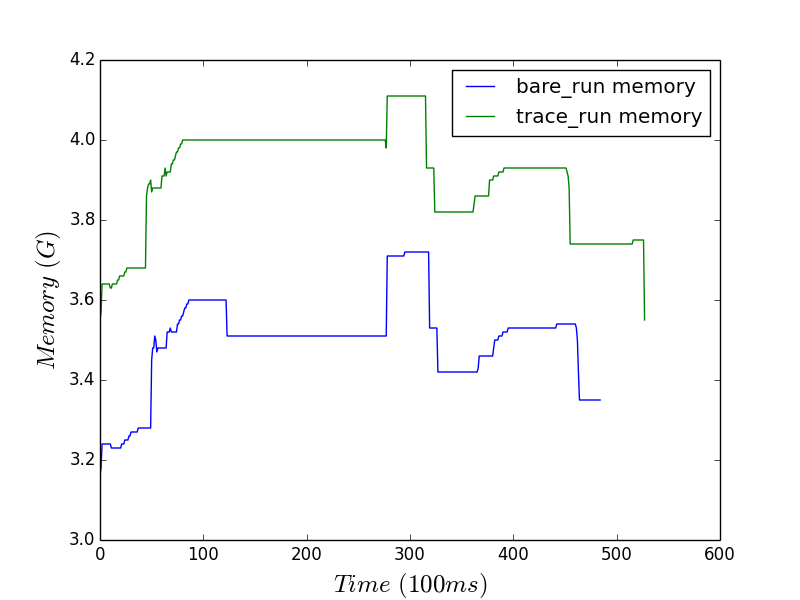
\includegraphics[width=1.0\linewidth]{ibench_memory_compare.png}
    \caption{Memory overhead with tracing.}
    \label{fig:ibench_memory_overhead}
\end{figure}

\begin{figure}[tb]
    \centering
    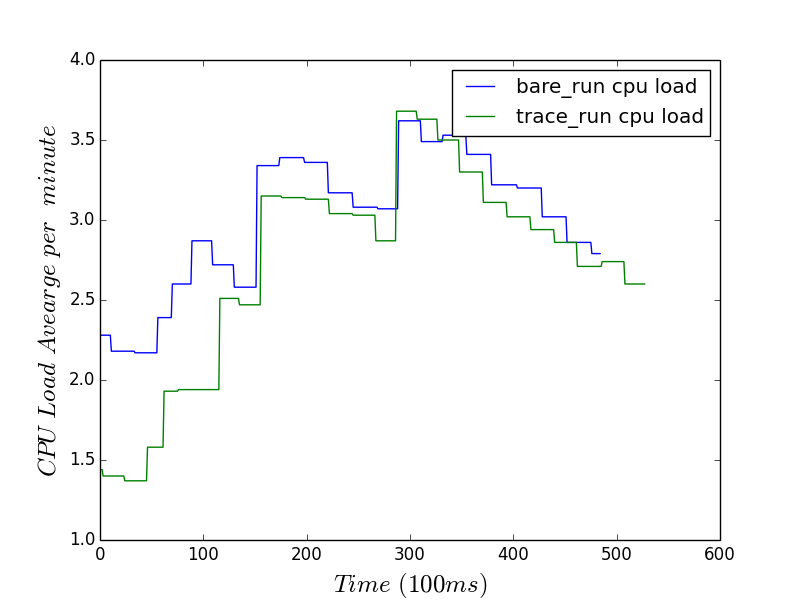
\includegraphics[width=1.0\linewidth]{ibench_cpuload_compare.png}
    \caption{CPU overhead with tracing.}
    \label{fig:ibench_cpu_overhead}
\end{figure}

\begin{itemize}
\item tracing overhead
	\begin{itemize}
	\item memory and CPU usage on top, while running ibench with and without our tracing enabled
	\item memory and CPU usage on top, while running the listed real world applications with and without our tracing enabled
	\item how much times it takes to filled the buffer we fixed 2G
	\item how many events recorded in the buffer
	\end{itemize}
\item number of edges and nodes in the graphs and portions of data the user need to examine to figure out the root cause.
\end{itemize}

\input{discussion}
\section{Related Work}
\label{sec:related-work}

While there is currently no system that can help users debug performance
issues in closed-source applications on proprietary macOS, several active
research topics are closely related.

\para{Event tracing.}
\begin{table}[ht]
\footnotesize
\centering
  \begin{tabularx}{\columnwidth}{l|XXX}
  \hline
Paradigm & Panappticon & AppInsight & \xxx\\
\hline
\hline
%User input & \mycheck & \mycheck & \mycheck \\
%Display update & \mycheck & \mycheck & \mycheck\\
Async calls & MessageQueue, & Upcall & libdispath\\
			& ThreadPoolExecutor &  & runloop \\
			&	&	&timer\\
IPC calls & \mycheck & \mycross & \mycheck \\
Batching & \mycross & \mycross & \mycheck \\
Data flag & \mycross & \mycross  & \mycheck \\
Wait-Wakeup & 4 primitives & Silverlight methods & system wide \\
%Fork & \mycheck & \mycorss & \mycross \\
%Interrupts &\mycross & \mycross &\mycheck\\
%Timeshare Maintain &\mycross &\mycross &\mycheck\\
%Syscall and backtrace
\hline
  \end{tabularx}
  \caption{Programming paradigms tracked.} 
  \label{table:paradigms}
\end{table}


Panappticon \cite{zhang2013panappticon} monitors a mobile system and uses the
trace to characterize the user transactions of mobile apps. Although it aims to
track system-wide events and correlate them without developer input, it supports
only two models of communication: work queue and thread pooling. AppInsight
\cite{ravindranath2012appinsight} instruments application to identify the
critical execution path in a user transaction. It supports the event callback
pattern, and does not trace across process or app boundaries.
Magpie~\cite{barham2004using} monitors server applications in Windows with the
goal to model the normal behaviors of a server application in response to a
workload. This model further helps detecting anomalies statistically. Magpie
requires a manual-written event schema for all involved applications to capture
precise request graphs, whereas \xxx has a simple, application-agnostic schema
for system-wide tracing and enables users to provide more application-specific
knowledge on demand.

Aguilela \cite{aguilera2003performance} uses timing analysis to correlate
messages to recover their input-output relations while treating the application
as a black box. XTrace, Pinpoint and \etc ~\cite{fonseca2007x, chen2002pinpoint,
chow2014mystery} trace the path of a request through a system using a unique
identifier attached to each request and stitch traces together with the
identifier. \xxx comes up violation patterns and does not assume the presence of
a unified identifier in closed-source, third-party applications, frameworks, and
libraries.


\para{Performance anomaly detection.}
Several systems detect performance
anomalies automatically. \cite{han2012performance, yuan2012conservative}
leverage the user logs and call stacks to identify the performance anomaly.
\cite{cohen2004correlating, saidi2008full, xu2009detecting, du2017deeplog}
apply the machine learning method to identify the unusual event sequence as an
anomaly. \cite{yu2014comprehending} generates the wait and waken graph from
sampled call stacks to study a case of performance anomaly.

These systems are orthogonal to \xxx as \xxx's goal is to diagnose an
already-detected performance anomaly. These systems can help \xxx by detecting
more accurately when a performance issue arises.

\section{Conclusion} \label{sec:conclusion}
Our key insight in this paper is that causal tracing is inherently
imprecise. We have reported patterns we observed that pose big precision
challenges to causal tracing, and built \xxx, a practical system for
effectively debugging performance issues in macOS applications despite the
imprecision of causal tracing.  To do so, it lets a user provide domain
knowledge interactively on demand. Our results show that \xxx effectively
helped us locate all root causes of the issues, including a bug in Chromium,
01 and incurred 12\% CPU overhead overall in its system-wide tracing.

\end{sloppypar}

\clearpage
% uncomment to tweak with bib spacing
%\setlength\bibsep{2.25pt}
{
%\small
 \bibliographystyle{abbrvnat}
 \bibliography{bib/biblio}
}

\end{document}
